\subsection{Presenza in Sede}
Dopo essersi autenticati è possibile registrare la propria presenza in sede scrivendo "Presenza" e il chatbot comunica l'avvio dell'operazione richiedendo il nome di una sede. 
Quindi si scrive il nome, se il nome fa parte della lista sedi viene accettato e il chatbot conclude l'operazione di registrazione presenza, altrimenti il bot comunica che la sede non è stata accettata e si invita a reinserire il nome. 
\subsubsection{Schermata Registrazione Presenza - Avvenuta con Successo}
\begin{figure}[H]
    \centering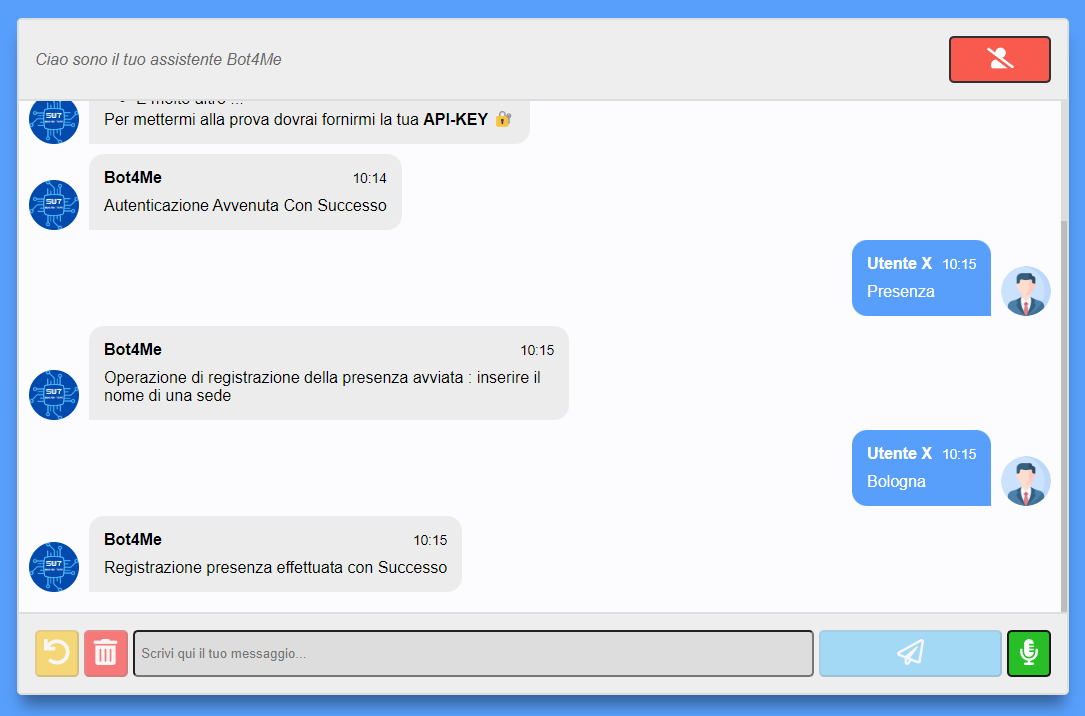
\includegraphics[width=0.9\textwidth, height=0.7\textheight, keepaspectratio]{images/schermata_presenza_successo.png}
    \caption{Schermata Dialogo Registrazione Presenza - Avvenuta con Successo}
\end{figure}

\subsubsection{Schermata Registrazione Presenza - Fallita}
\begin{figure}[H]
    \centering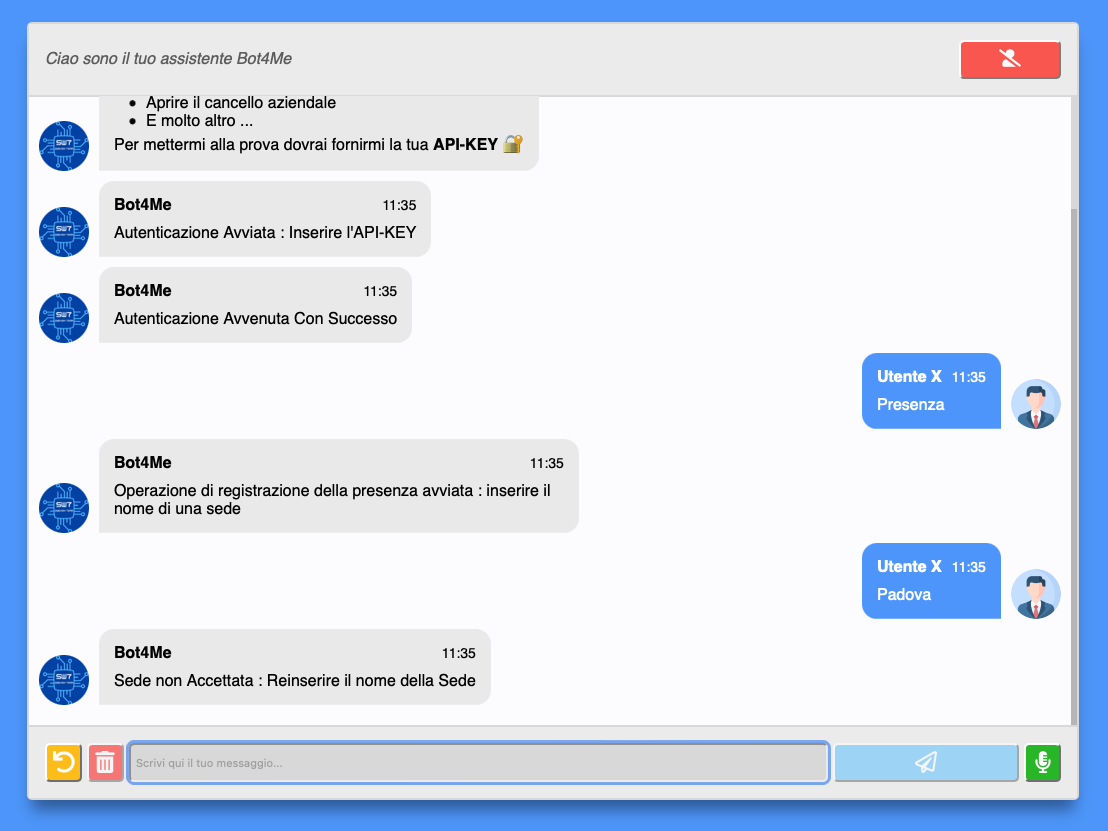
\includegraphics[width=0.9\textwidth, height=0.7\textheight, keepaspectratio]{images/schermata_presenza_fallita.png}
    \caption{Schermata Dialogo Registrazione Presenza - Fallita}
\end{figure}